
% You need to select the LuaTeX engine to compile to pdf
% If you use Overleaf, you have to change the compiler (https://www.overleaf.com/learn/how-to/Changing_compiler)
% Reason: The common pdfTeX engine cannot use system fonts: Calibri, Georgia


\documentclass[aspectratio=169]{beamer}
%  aspect-ratios "43" and "169", and "smaller" or "9pt" should work

% Load package "amsmath" before PSI43 (because "fontspec" inside PSI43 should be loaded before "amsmath" according to an advice)
\usepackage{amsmath}

\usepackage[blockcolored]{PSI43} % blockcolored is required if you want to have colored blocks, because the default beamer theme has uncolored boxes



\begin{document}

\title{A novel approach to energy system analysis and technology assessment}

\author[L.~Wittgenstein]{Ludwig Wittgenstein}
% if short author is given as an option, it will be taken for the footline

\institute[LEA, PSI]{Laboratory of Energy Systems Analysis, Paul Scherrer Institute}
% if short institute is given as  an option, it will be taken for the footline

\subtitle{\textbf{1st line of subtitle}\\2nd line (different no of lines move the gray box at correct position. Empty line:  $\sim$\textbackslash\textbackslash)}

\date{LEA Seminar, 1.1.2021} % can be left empty


\begin{frame}[plain] % plain prohibits logo, footer etc.
  \titlepage
\end{frame}


\begin{frame}{A list that is revealed}  
  \begin{itemize}
  \item<1-> Item 1
  \item[-]<1->  Item 1 (with dash instead of bullet)
    \begin{itemize}
    \item[1.]<1-> Item 1a
    \item[2.]<1-> Item 1b
    \end{itemize}
  \item<2->  Item 2 (revealed on next slide)
  \item<3-> Item 3
    \begin{itemize}
    \item<3-> Item 4
      \begin{itemize}
      \item<3-> Item 5
      \end{itemize}
    \end{itemize}
  \end{itemize}
 \vspace*{\fill} % to put the text a little bit upwards
\end{frame}



\begin{frame}[squeeze]{Titles over two lines are possible\\
    (PSI logo goes to 2nd line)}
  Some formulas, which can be tagged, e.g.\ \thetag{$\ast$}:
  \begin{align*}
    a + b  & = \int_a^b f(x)\,dx             && \tag{$\ast$}\\
    \sum_{n=1}^N x_{i_n} &= \frac{a+b}{c+d}  &&
  \end{align*}
  \begin{itemize}
  \item  $\alpha = \zeta$, bold: $\boldsymbol{\alpha} = \boldsymbol{\zeta}$ 
  \item $\mathcal{F}_t$, $\mathbb{R}^n$
  \item $\{t \mid t=1,\dots,T\}$
  \item $f\colon X\to Y$; $f\colon x\mapsto y$
  \end{itemize}
   \alert{This is a frame with the usual `squeeze' option of beamer to narrow linespacing a little bit; the color of this text is called \texttt{alert} in beamer}
  
  \structure{This is a color predefined in beamer called \texttt{structure}}
\end{frame}

\begin{frame}{Columns and Blocks}
  You can start text very high with a space command \texttt{\textbackslash PSIfill} (see the .tex file of this presentation)

 The default beamer theme has uncolored blocks. The option \texttt{blockcolored} was set in the package for coloring: 
  \begin{columns}
    \begin{column}[T]{0.6\linewidth}
      \begin{block}{Text in block title}
        Text in block in first column
      \end{block}
      \begin{exampleblock}{Title text of example block}
        Text in block in first column
      \end{exampleblock}
      Text outside of block in first column
    \end{column}
    \begin{column}[T]{0.4\linewidth}
      \begin{block}{Title text in block}
        Text in second column 
      \end{block}
      \begin{alertblock}{Text in an alert block}
        Text in second column
      \end{alertblock}
      \begin{block}{}
        This is a block without title (not nice)
      \end{block}
    \end{column}
  \end{columns}
    
    \PSIfill
 \end{frame}
 

 \begin{frame}{Title}
   \PSIvspace
  You can start text at the gray box with the command \texttt{\textbackslash PSIspace} and \texttt{\textbackslash PSIfill} (see the .tex file)
  \begin{figure}
    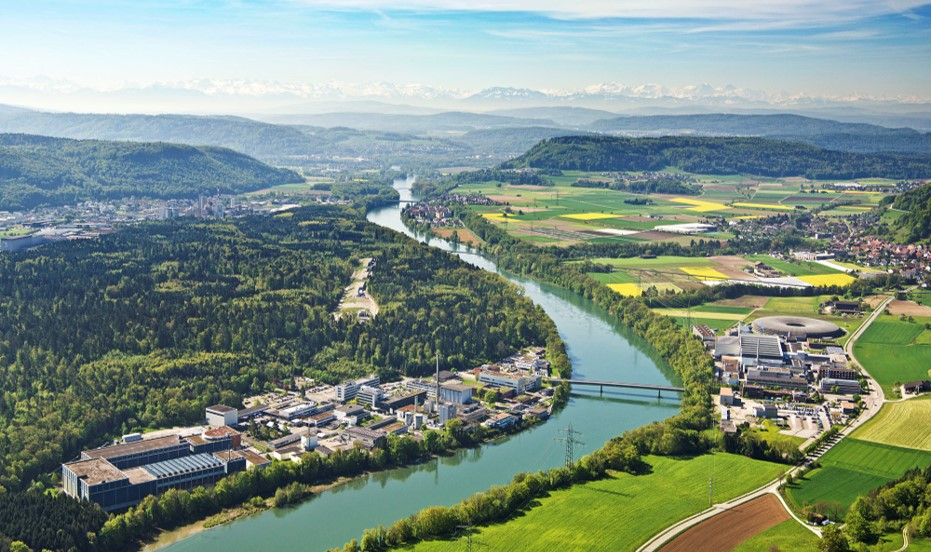
\includegraphics[width=0.3\pagewidth]{PSIlandscape43}
    \caption{Figures are automatically centered in beamer}
    \label{fig:PSI}
  \end{figure}

     \PSIfill
\end{frame}

\begin{frame}{Overwrite the margins}
You can overwrite the margins with a wide column:
  \begin{columns}
  \begin{column}{1.18\linewidth}
    \colorbox{structure!10}{
      \begin{minipage}[t][0.8\textheight][t]{\textwidth}
        this is a very long text that needs a lot of space this is a very long text that needs a lot of space this is a very long text that needs a lot of space 
      \end{minipage}}
  \end{column}
\end{columns}
\end{frame}

\PSItrailer{Wir schaffen Wissen -- heute für morgen}{
    \textbf{My thanks go to}
     \smallskip
    \begin{itemize}
    \item Co-author 1
    \item Co-author 2 who has a very long name 
    \item Supervisor 1
    \item Supervisor 2  
    \end{itemize}
    }
  

\end{document}

% The following can be deleted if not the EMACS editor is used for editing

%%%Local Variables:
%%% mode: latex
%%% TeX-master: t
%%% TeX-engine: luatex
%%% End:
